\chapter{Introduction}\label{intro}

Ce chapitre présente les caractéristiques principales du code, à savoir les langages utilisés
(cf. ~\ref{intro.langages}), le type d'architecture général (cf. ~\ref{intro.archi}) et 
l'arborescence des dossiers qui composent le site (cf. ~\ref{intro.folders}).

\section{Langages utilisés}\label{intro.langages}

Le code de PAG fait intervenir 5 langages différents couramment utilisés dans le développement 
web. Pour les lecteurs moins familiers avec le développement web, le 
tableau~\ref{intro.tab.langages} ci-contre récapitule ces langages et l'utilité de chacun à 
titre d'information.

\begin{table}[h]
\begin{center}
\begin{tabular}{|l|l|l|}
  \hline
  \textbf{Langage} & \textbf{Acronyme} & \textbf{Utilité} \\
  \hline
  \textbf{HTML} & \textit{\underline{H}yper\underline{T}ext \underline{M}arkup \underline{L}anguage} & Structure des pages\\
  \hline
  \textbf{CSS} & \textit{\underline{C}ascade \underline{S}tyle \underline{S}heet} & Style des pages\\
  \hline
  \textbf{PHP} & \textit{\underline{P}HP: \underline{H}ypertext \underline{P}reprocessor} & Traitement des requêtes\\
  \hline
  \textbf{SQL} & \textit{\underline{S}tructure \underline{Q}uery \underline{L}anguage} & Gestion de la base de données\\
  \hline
  \textbf{JavaScript} & Aucun & Interactivité des pages\\
  \hline
\end{tabular}
\end{center}
\vspace{-0.5cm}
\caption{Langages utilisés.}
\label{intro.tab.langages}
\end{table}

Il est utile de préciser aussi, à ce stade, que la partie JavaScript utilise le \textit{framework} 
\jquery~\footnote{Cf. \url{https://jquery.com/}}, principalement à des fins de compatibilité avec 
tous les navigateurs Web répandus (bien que \jquery facile aussi l'écriture du code).

\section{Architecture}\label{intro.archi}

La conception de PAG vise à appliquer autant que faire se peut l'architecture 
\textbf{MVC}\footnote{Cf. \url{https://fr.wikipedia.org/wiki/MVC}}, 
c.-à-d. \textit{\underline{M}odèle - \underline{V}ue - \underline{C}ontrôleur}, illustrée à 
la figure~\ref{fig.concept.MVC}. Cette architecture 
vise à séparer clairement le code qui va représenter les données (le modèle), le code qui va 
fournir une interface à l'utilisateur (la vue) et le code qui va gérer la logique des opérations 
réalisées par l'utilisateur (le contrôleur).

\begin{center}
    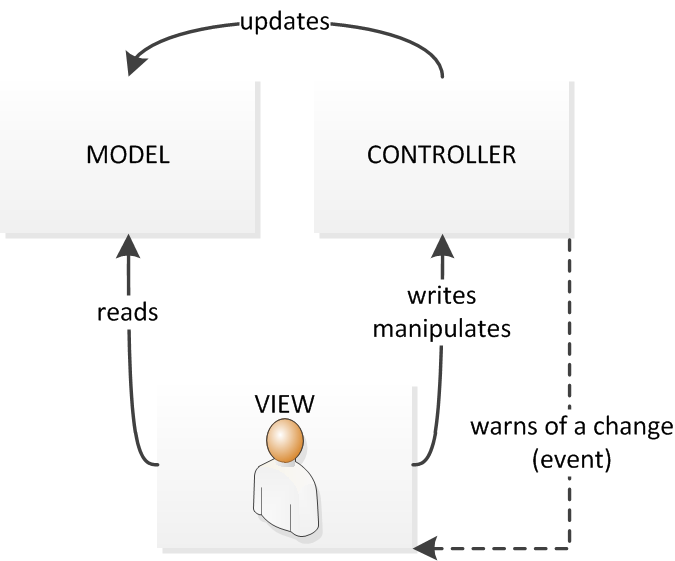
\includegraphics[scale=1.0]{figures/ModeleMVC.png}
	\captionof{figure}{Vue conceptuelle du \textit{design pattern} MVC (source: Wikipédia)}
	\label{fig.concept.MVC}
\end{center}

Dans le cas de PAG, en pratique, le modèle rassemble un ensemble de classes PHP qui vont servir 
d'abstraction pour le contenu de la base de données, tandis que la vue est constituée d'une part 
d'un ensemble de sous-dossiers qui vont isoler les fichiers écrits dans certains langages (ici, 
le CSS et le JavaScript) et d'autre part d'un ensemble de \textit{templates} et % TODO: ref vers un autre chapitre 
de fonctions d'interprétation intermédiaire qui vont isoler le code HTML et son agencement selon 
l'utilisateur du reste du site. Reste alors les scripts principaux, écrits en PHP et situés 
majoritairement à la racine du site, qui s'apparentent à la partie contrôle et qui se veulent le 
plus haut niveau possible (c.-à-d., en reléguant les aspects plus techniques à d'autres parties du 
code). Un détail des sous-dossiers est donné à la section~\ref{intro.folders}.

En pratique, cela veut dire que les scripts principaux (écrits en PHP)
\begin{itemize}
\item ne contiennent aucune requête SQL explicite, et mentionnent tout au plus les débuts et les 
fins de transactions avec la base de données (c.-à-d. une suite logique de requêtes qu'on doit 
pouvoir annuler si l'une d'entre elles échoue et compromet l'intégrité des données), 
\item ne comportent pas ou peu de CSS ou de JavaScript, se contentant de lister les fichiers 
écrits dans ces langages qui seront utilisés pour créer le rendu de la page finale et gérer son 
interactivité, 
\item ne comportent pas non plus de HTML ou très peu, celui-ci étant écrit pour la majeure 
partie dans des \textit{templates} isolés dans la partie \textit{vue} du code.
\end{itemize}
\vspace{0.3cm}
Il ne reste alors que la logique "\textit{haut-niveau}" qui va régir les actions de l'utilisateur. 
Pouvoir isoler cette logique du reste du code est très important pour sa lisibilité: comme les 
lecteurs du code pourront s'en apercevoir, certaines pages manipulent plusieurs fonctionnalités 
(assez souvent optionnelles) d'un coup. S'il est tout à fait possible de reproduire tout un script 
en mélangeant tout à la fois le PHP, le HTML, le CSS et le JavaScript, le résultat serait beaucoup 
plus verbeux et confus à la lecture. % TODO: ref vers un autre chapitre

\section{Arborescence des dossiers}\label{intro.folders}

Le tableau~\ref{intro.tab.folders} reprend les principaux dossiers et leur contenu.

\newpage % Pour avoir les footnotes du tableau sur la meme page

\begin{savenotes}
\begin{table}[!t]
\begin{tabular}{|l|p{0.75\textwidth}|}
  \hline
  \textbf{Dossier} & \textbf{Contenu} \\
  \hline
  \texttt{./} (racine) & Contient les scripts principaux, écrits en PHP, qui correspondent à la 
                         partie \textbf{\textit{Contrôle}} du code. Une poignée d'images par 
                         défaut sont également présentes.\\
  \hline
  \texttt{ajax/} & Contient les scripts PHP qui traitent les requêtes asynchrones envoyées à 
                   l'aide de JavaScript, utilisées pour gérer l'interaction entre la page web et 
                   l'utilisateur sans rechargement de celle-ci. Le dossier est nommé d'après le 
                   nom donné à ce type d'architecture: \textbf{Ajax} (pour 
                   \textit{\underline{a}synchronous \underline{J}avaScript \underline{a}nd 
                   \underline{X}ML}~\footnote{\url{https://fr.wikipedia.org/wiki/Ajax\_(informatique)}}).\\
  \hline
  \texttt{javascript/} & Contient, comme son nom l'indique, tous les fichiers JavaScript du site. 
                         Cela inclut la librairie \jquery, mais aussi un fichier 
                         \texttt{default.js} chargé sur toutes les pages et comportant les 
                         fonctionnalités JavaScript les plus courantes et essentielles.\\
  \hline
  \texttt{libraries/} & Contient des librairies de fonctions écrites en PHP, notamment celles qui 
                        sont utilisées pour gérer les \textit{uploads}. La librairie la plus 
                        essentielle est \texttt{Header.lib.php}: elle sert de base commune à tous 
                        les scripts. Le chapitre~\ref{headerlib} revient en détails sur ce qu'elle 
                        fournit.\\% TODO
  \hline
  \texttt{model/} & Contient des classes PHP qui modélisent chacune des entités stockées dans la 
                    base de données. Leur but est de rassembler les requêtes SQL associées à une 
                    même entité (et leur traitement) dans le script PHP qui y correspond. Ce 
                    sous-dossier correspond donc à la partie \textbf{\textit{Modèle}} du code.\\
  \hline
  \texttt{res\_icons/} & Contient toutes les icônes utilisées sur le site. Toutes celles-ci sont 
                        libres de droit (et proviennent de sources tel 
                        \textit{IconsDB}~\footnote{\url{https://www.iconsdb.com/}}.\\
  \hline
  \texttt{style/} & A l'instar de \texttt{javascript/}, ce sous-dossier contient tous les fichiers 
                    écrits dans un même langage, ici le CSS. C'est dedans que se trouve l'ensemble 
                    des fichiers de style du site. En particulier, le fichier \texttt{default.css} 
                    contient du style utilisé sur toutes les pages du site (sinon la plupart).\\
  \hline
  \texttt{upload/} & Ce sous-dossier ne contient pas de ressource ou de code, mais sert à stocker 
                     les \textit{uploads} des utilisateurs. Un sous-dossier \texttt{uploads/tmp/} 
                     stocke les fichiers temporaires de chaque utilisateur (un sous-dossier par 
                     utilisateur).\\
  \hline
  \texttt{view/} & Ce dernier sous-dossier correspond à la partie \textbf{\textit{Vue}} du code. 
                   Sa racine contient les fichiers \texttt{Header.inc.php} et 
                   \texttt{Footer.inc.php} qui encadrent toutes les pages du site.\\ % TODO: ref vers un autre chapitre
  \hline
\end{tabular}
\caption{Description de l'arborescence des dossiers principaux.}
\label{intro.tab.folders}
\end{table}
\end{savenotes}
